\subsection{Topology} \label{subsec:ecat-topology}

\emph{EtherCAT} supports a variety of network topologies like \emph{line}, \emph{tree}, \emph{star} or \emph{daisy-chain}.
Many ESCs and I/O modules already include ports to create network branches, which eliminates the need to use switches or any other type of infrastructure components.
Regardless, classical \emph{Ethernet} star topology can be used to implement an \emph{EtherCAT} network.
When designing a certain network, multiple topologies can be combined into a hybrid topology network.
\autoref{fig:ecat-topology} (page \pageref{fig:ecat-topology}) presents a possible illustration of such case.

\begin{figure}[htp]
	\centering
	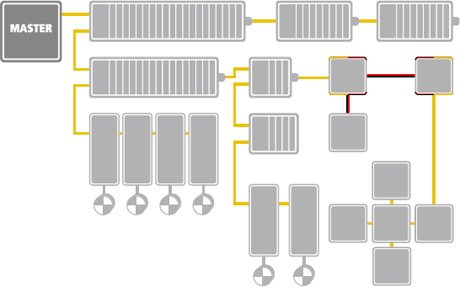
\includegraphics[width=\textwidth]{EtherCAT_Technology_03_Topology.jpg}
	\caption{Example of a hybrid topology EtherCAT network \cite{protocol:ethercat}}
	\label{fig:ecat-topology}
\end{figure}

ESCs also include support for a ``Hot Connect'' feature which means existing nodes can be removed and new nodes can be added to the network during runtime.
The controllers can detect these changes in a very short time (typically less than 15$\mu$s), allowing a smooth state transition without interfering with the rest of the network.

There is also a big flexibility in terms of available cabling option, from inexpensive industrial \emph{Ethernet} cables to fiber optics, having the entire Ethernet wiring possibilities available for use.

EtherCAT gateways provide the means to incorporate other fieldbus networks as a subnetwork.
This allows a gradual changeover between fieldbuses by keeping network sections that may contain components which still do not support the EtherCAT interface.

Due to the fact that EtherCAT uses a 16-bit address length, up to $65535$ devices can exist in a single network segment, which makes scalability virtually unlimited.
This large device count removes the need to use bus extension methods, like traditional gateways, providing even the largest EtherCAT networks the best possible performance, without unnecessary delays.
